\begin{wrapfigure}[20]{r}{7.5cm}
\caption{Feature Correlation Plot}
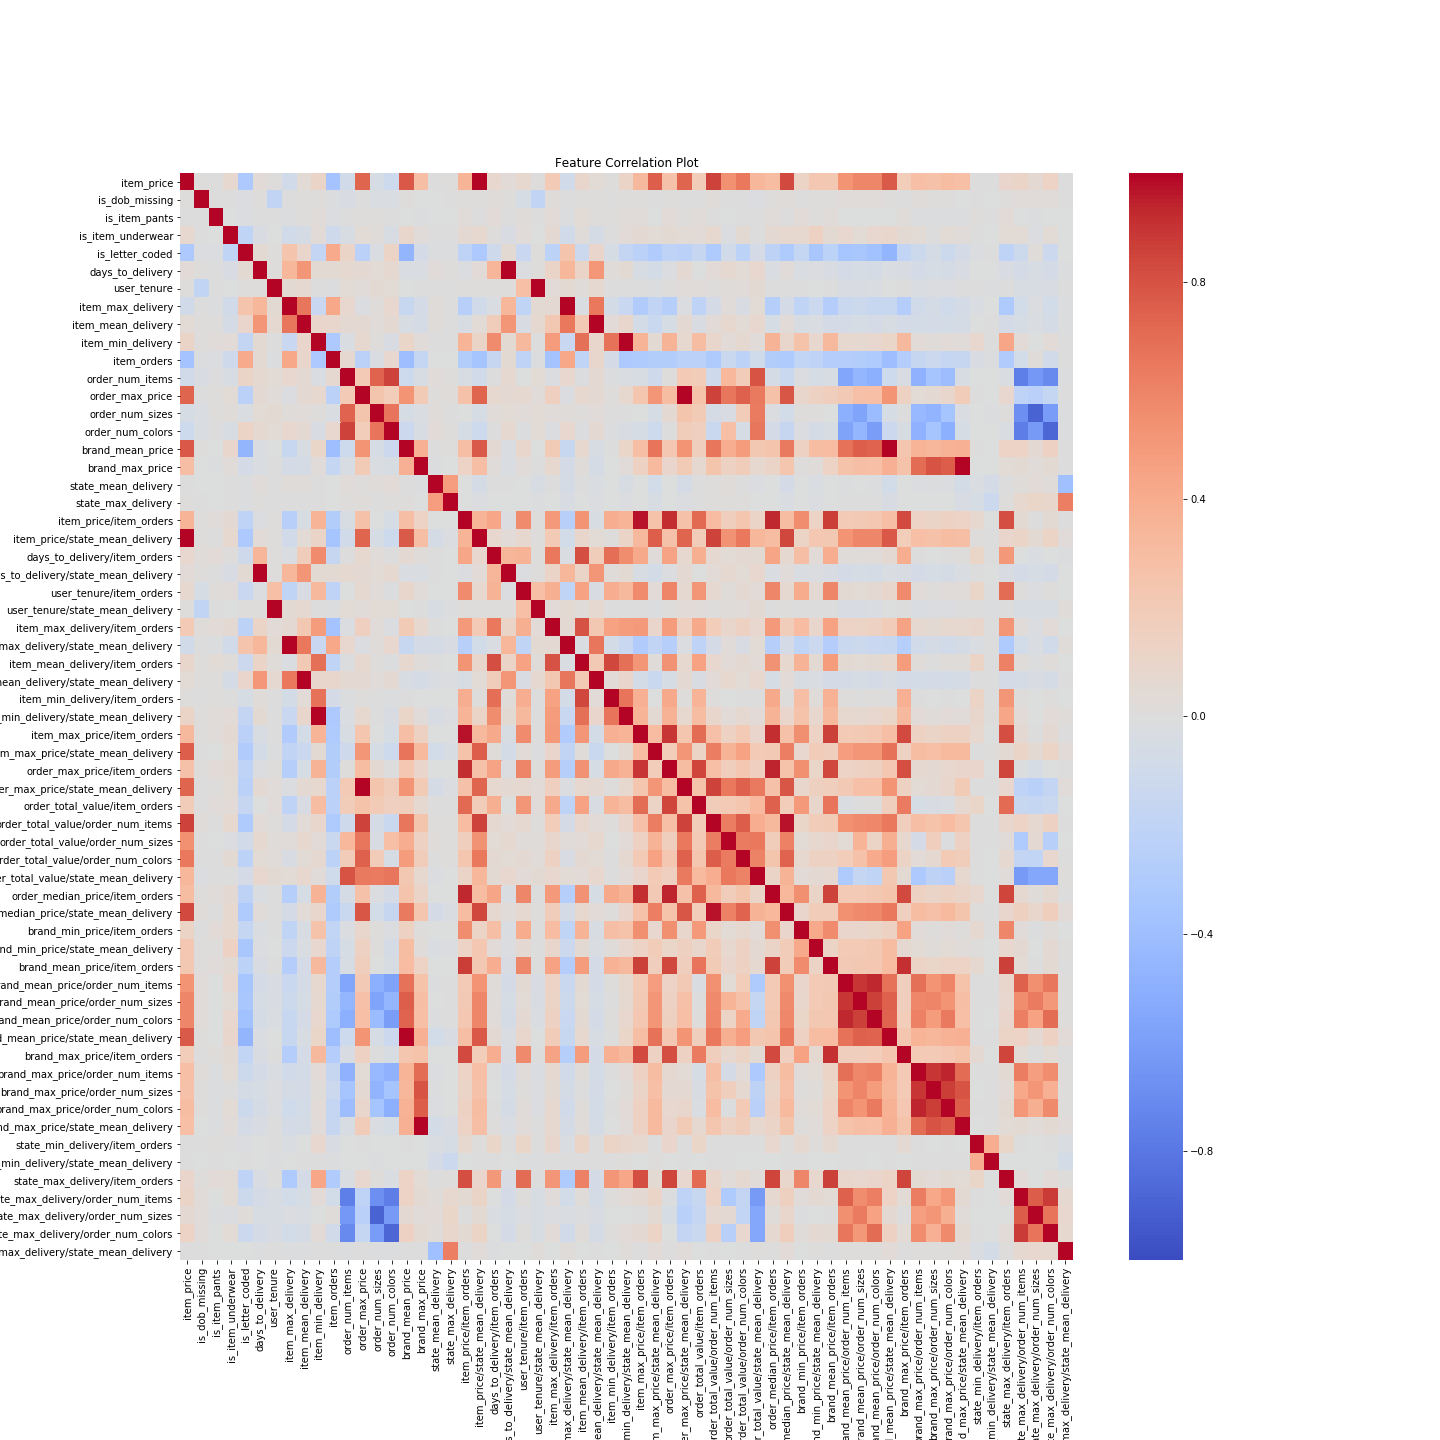
\includegraphics[scale=0.28]{../eda/corrplot.png}
\end{wrapfigure}

The data contained numerous missing values. Some of these were obscured by unorthodox codes, specifically for the delivery date it seemed that dates lying as far back as 1994 were being used to encode a missing value. However, once encountered, these missing values were easy to impute by the mean number of days passed between the order and the delivery of the item for cases were the delivery date was available. When looking at the distribution of days between order and delivery it seemed more in order to use the median since it was heavily skewed, yet imputing by the mean seemed provide better results. Similarly, for some users it was difficult to compute their age, since they either did not provide their day of birth or instead opted to provide implausible ones. Consequently, all years of birth lying farther back than 1926 were removed and the age of these users was imputed by the difference in days between registration date and the birth date, of the valid users which was subtracted from the registration date of the incredulous ones.

The data contained a large number of categorical variables which in turn contained numerous levels. Especially the items' colors involved some spelling mistakes and extravagant names for different shades of the same color. Both problems were solved by manually sifting through the various labels and summarizing the more detailed color names into broader categories. This way it was able to reduce the 85 initial colors to 14 unique levels in the cleaned data. For these densely populated categories it was possible to calculate the Weight of Evidence \cite{woe}.

\begin{table}
\centering
\caption{Selection of engineered features}
\label{features-tab}
\begin{tabular}{@{}lll@{}}
       & feature             & description                           \\ \midrule
users  & \texttt{tenure}              & days between registration and order        \\
items  & \texttt{price-off}           & discount compared to maximum item price    \\
orders & \texttt{num items}           & count of item IDs in order                 \\
       & \texttt{days until delivery} & days between order and delivery            \\
       & \texttt{num sizes}           & count of unique sizes                      \\
       & \texttt{total value}         & sum of all item prices in order            \\
       & \texttt{num colors}          & count of unique colors                     \\
       & \texttt{seq number}          & enumerate order date per user              \\
brands & \texttt{brand mean price}    & average price of item's brand              \\
state  & \texttt{state mean delivery} & average number of days until delivery
\end{tabular}
\end{table}

The items' sizes proved to be difficult to clean. Ideally one would want to extract categories like \textit{small}, \textit{medium}, \textit{large} and while these are provided in some, they are not provided in the majority of cases. Instead there is a whole clutter of different sizes and without knowing the type of clothing only limited information can be extracted. Through the use of regular expressions, for example, it is possible to determine if items are pants, since they have exactly four numerical digits (two for the width and two for the length).

Table \ref{features-tab} contains a selection of the most important engineered features. Furthermore, all possible pairwise ratios and interaction terms were computed where the most correlated features were discarded afterwards.

Finally, a Random Forest was trained, in order to extract the most important features out of the 163 that were generated. Subsequently the 20 most influential variables were picked based on their variable importance for further modelling.